\documentclass[
    classnum=MATH564,
    classname=MATHEMATICAL\ MODELING,
    due=January\ 28\,\ 2020,
    author=Gabrielle\ Streeter\qquad Hannah\ Wu\qquad\ Minghang\ Li,
    authorshort=Streeter\ \&\ Wu\ \&\ Li,
    teacher= Zachary\ M.\ Boyd,
    hw=1
]{hw-template}

\renewcommand{\theenumi}{(\alph{enumi})}
\newcommand{\requiregraph}{\colorbox{yellow}{\{GRAPH NEEDED\}}}
\newenvironment{Figure}
  {\par\medskip\noindent\minipage{\linewidth}}
  {\endminipage\par\medskip}

% ============================================================================ %

\begin{document}

\begin{center}
    \bigskip
    \LARGE
    \textbf{MATH PART}
    \bigskip
\end{center}

% Problem 1
\begin{homeworkProblem}
Consider the difference equation
\[
    x_{n+2} - 3x_{n+1} + 2x_n = 0.
\]
\begin{enumerate}
    \item Show that the general solution to this equation is
    \[
        x_n = A_1 + 2^n A_2
    \]
    Now suppose that $x_0 = 10$ and $x_1 = 20$. Then $A_1$ and $A_2$ must
    satisfy the system of equations
    \[
        \begin{aligned}
            A_1 + 2^0 A_2 = x_0 = 10,\\
            A_1 + 2^1 A_2 = x_1 = 20.
        \end{aligned}
    \]
\item Solve for $A_1$ and $A_2$ and find the solution to the above
\textit{initial value problem}.
\end{enumerate}

\segline

\solution

% Write your answers here %
\begin{enumerate}
    \item The characteristic solution is \[
        \lambda^2 - 3 \lambda + 2 = 0
    \]
    The characterictic roots are \[
        \lambda_1 = 1, \quad \lambda_2 = 2.
    \]
    By the principle of linear superposition, the general solution is indeed \[
        x_n = A_1 + 2^n A_2
    \]
    \item Solving the system of equations
    \[
        \begin{aligned}
            A_1 + 2^0 A_2 = x_0 = 10,\\
            A_1 + 2^1 A_2 = x_1 = 20.
        \end{aligned}
    \] gives \[
        A_1 = 0, \quad A_2 = 10.
    \]
    Therefore, the solution should be \[
        x_n = 10 \cdot 2^n
    \]
\end{enumerate}
\end{homeworkProblem}

\pagebreak

% Problem 2
\begin{homeworkProblem}
Solve the following difference equations subject to the specified $x$ values and
sketch the solutions:
\begin{enumerate}
    \item $x_n - 5x_{n-1} + 6x_{n-2} = 0;\quad x_0 = 2, x_1 = 5.$
    \addtocounter{enumi}{1}
    \item $x_n - x_{n-2} = 0;\quad x_1 = 3, x_2 = 5.$
    \addtocounter{enumi}{1}
    \item $x_{n+2} + x_{n+1} - 2x_n = 0; \quad x_0 = 6, x_1 = 3.$
\end{enumerate}

\segline

\solution

\begin{enumerate}
    \item The characterictic function is \[
        \lambda^2 - 5\lambda + 6 = 0
    \]
    The characterictic roots are \[
        \lambda_1 = 2, \quad \lambda_2 = 3.
    \]
    The general solution should be \[
        A_1 2^n + A_2 3^n  = 0.
    \]
    Plug in $x_0 = 2$ and $x_1 = 5$, we have \[
        \left\{
        \begin{aligned}
            &A_1 + A_2  = 2\\
            &2A_1  + 3A_2 = 5
        \end{aligned}
        \right.
        \quad
        \Rightarrow
        \quad
        \left\{
        \begin{aligned}
            A_1 = 1\\
            A_2 = 1
        \end{aligned}
        \right.
    \]
    To sum up, the specific solution should be $$
        x_n = 2^n + 3^n.
    $$
    And the plot would look like
    \begin{Figure}
        \centering
        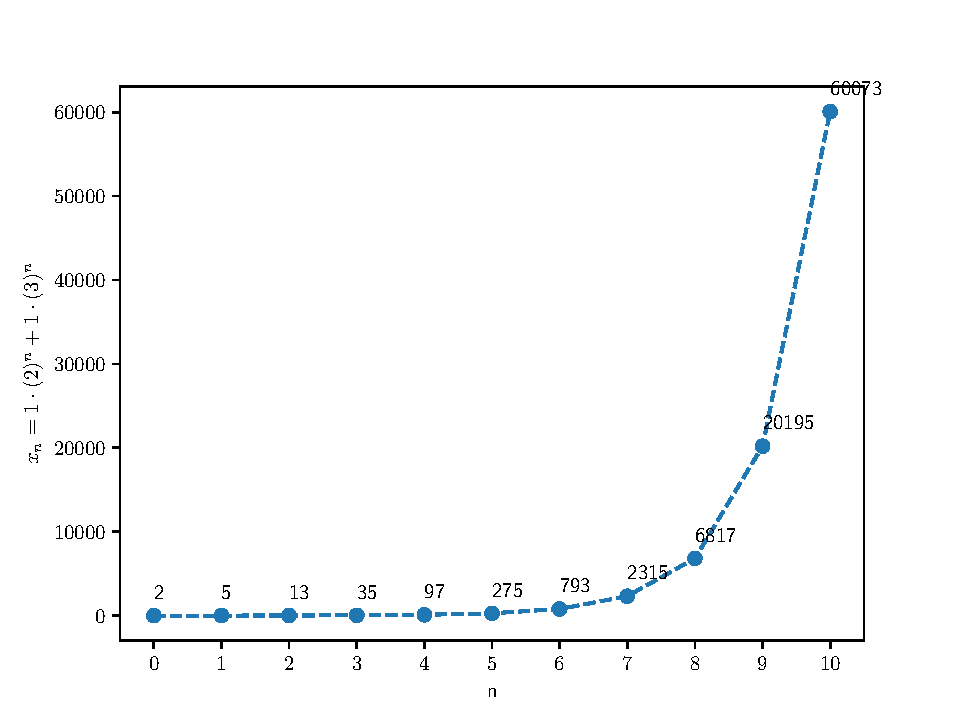
\includegraphics[scale=0.5]{media/hw1/fig2(a).pdf}
    \end{Figure}
    \addtocounter{enumi}{1}

    \item The characterictic function is \[
        \lambda^2 - 1 = 0
    \]
    The characterictic roots are \[
        \lambda_1 = -1, \quad \lambda_2 = 1.
    \]
    The general solution should be \[
        A_1 (-1)^n + A_2  = 0
    \]
    Plug in $x_1 = 3$ and $x_2 = 5$, we have \[
        \left\{
        \begin{aligned}
            &-A_1 + A_2  = 3\\
            &A_1  + A_2 = 5
        \end{aligned}
        \right.
        \quad
        \Rightarrow
        \quad
        \left\{
        \begin{aligned}
            A_1 = 1\\
            A_2 = 4
        \end{aligned}
        \right.
    \]
    To sum up, the specific solution should be $$
        x_n = (-1)^n + 4.
    $$
    And the plot would look like
    \begin{Figure}
        \centering
        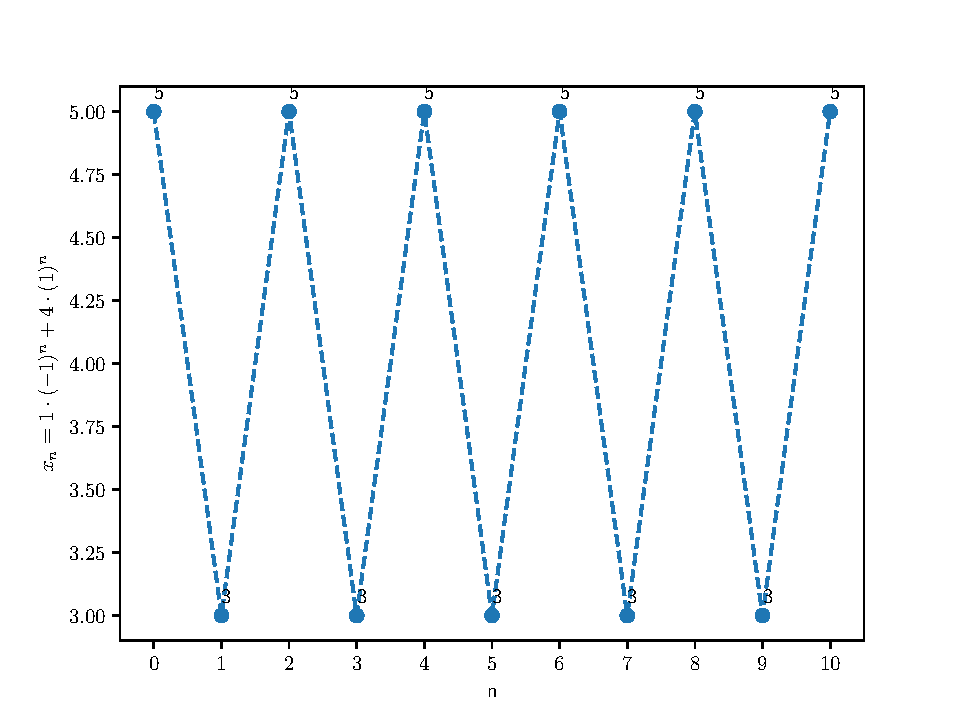
\includegraphics[scale=0.5]{media/hw1/fig2(c).pdf}
    \end{Figure}
    \addtocounter{enumi}{1}
\pagebreak
    \item The characterictic function is \[
        \lambda^2 + \lambda -2 = 0
    \]
    The characterictic roots are \[
        \lambda_1 = 1, \quad \lambda_2 = -2.
    \]
    The general solution should be \[
        A_1 + A_2 (-2)^n = 0
    \]
    Plug in $x_0 = 6$ and $x_1 = 3$, we have \[
        \left\{
        \begin{aligned}
            &A_1 + A_2  = 6\\
            &A_1 - 2A_2 = 3
        \end{aligned}
        \right.
        \quad
        \Rightarrow
        \quad
        \left\{
        \begin{aligned}
            A_1 = 5\\
            A_2 = 1
        \end{aligned}
        \right.
    \]
    To sum up, the specific solution should be $$
        x_n = (-2)^n + 5.
    $$
    And the plot would look like
    \begin{Figure}
        \centering
        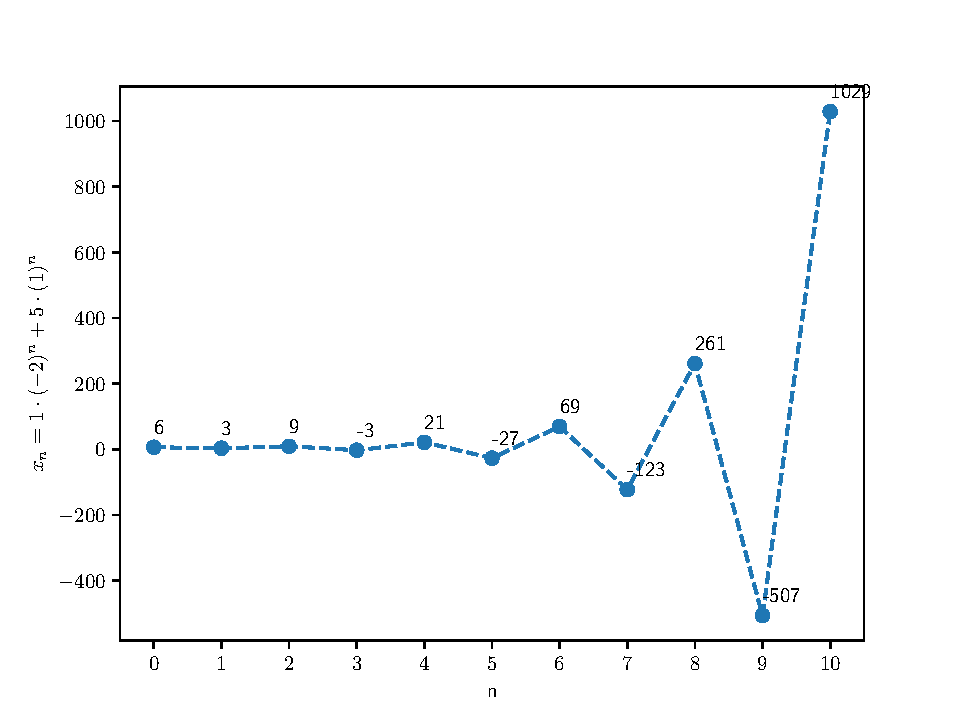
\includegraphics[scale=0.5]{media/hw1/fig2(e).pdf}
    \end{Figure}
\end{enumerate}

\end{homeworkProblem}

\pagebreak

% Problem 3
\begin{homeworkProblem}
\begin{enumerate}
    \item In Section 1.3 it was shown that the general solution to equation
    (16a, b) is (22) provided $\lambda_1 \neq \lambda_2$. Show that if
    $\lambda_1 = \lambda_2 = \lambda$ then the general solution is
    \[
        A_1\lambda^n + A_2 n \lambda^n.
    \]
    \item Solve and graph the solutions to each of the following equations or
    systems
    \begin{enumerate}[label=(\roman*)]
        \addtocounter{enumii}{1}
        \item $x_{n+2} - 2x_{n+1} + x_n = 0,$
        \item $x_{n+1} = -3 x_n - 2y_n,$\\
        $\qquad y_{n+1} = \phantom{-} 2 x_n +\phantom{2}y_n.$
    \end{enumerate}
\end{enumerate}

\segline

\solution
\begin{enumerate}
    % Solution 3(a)
    \item \textit{Proof} by Mathematical Induction:
    We know from (16a, b) that
    \[
        x_{n+2} = B_1 x_{n+1} + B_2 x_{n}
    \]
    is true for all $n$, where $B_1$ and $B_2$ are some constants.
    Suppose that $\lambda_0$ is the repeated solution to the characteristic
    equation
    \[
        \lambda^2 - B_1 \lambda - B_2 = 0
    \]
    By Vieta's formulas, we know that $B_1 = 2\lambda_0$ and $B_2=-\lambda_0^2$.

    Suppose that the general solution formula is true for all integers from $0$
    through $k$, then we have\[
    \begin{aligned}
        x_k &= A_1 \lambda_0^k + A_2 k \lambda_0^k,\\
        x_{k-1} &= A_1 \lambda_0^{k-1} + A_2 (k-1) \lambda_0^{k-1}.
    \end{aligned}
    \]
    For $x_{k+1}$, we have \[
        \begin{aligned}
            x_{k+1} &= B_1 x_{k} + B_2 x_{k-1}\\
            &= B_1 (A_1 \lambda^k + A_2 k \lambda^k) +
            B_2 (A_1 \lambda^{k-1} + A_2 (k-1) \lambda^{k-1})\\
            &= A_1 (B_1 \lambda^k + B_2 \lambda^{k-1}) +
            A_2 (B_1 k \lambda^k + B_2 (k-1) \lambda^{k-1})\\
            &= A_1 (2\lambda^{k+1} - \lambda^{k+1}) +
            A_2 (2k\lambda^{k+1} + (1-k) \lambda^{k+1})\\
            &= A_1 \lambda^{k+1} + A_2 (k+1) \lambda^{k+1}
        \end{aligned}
    \]
    The truth of $x_0$ and $x_1$ is automatic since $A_1$ and $A_2$ are numbers
    selected intentionally to make the following equations true: \[
        x_0 = A_1, \quad x_1 = (A_1 + A_2) \lambda.
    \]
    \begin{flushright}
        $\qed$
    \end{flushright}

    \pagebreak
    % Solution 3(b)
    \item Note: the constants $A_1$ and $A_2$ are se as $1$ for both questions.
    \begin{enumerate}[label=(\roman*)]
    \addtocounter{enumii}{1}
    % Solution 3(b)(ii)
        \item The characteristic equation is \[
            \lambda^2 - 2\lambda + 1 = 0.
        \]
        So the roots should be $\lambda_1 = \lambda_2 = \lambda = 1$.
        The general solution would be \[
            x_n = A_1 + A_2 n,
        \] since the power of $1$ is always $1$.
        \begin{Figure}
            \centering
            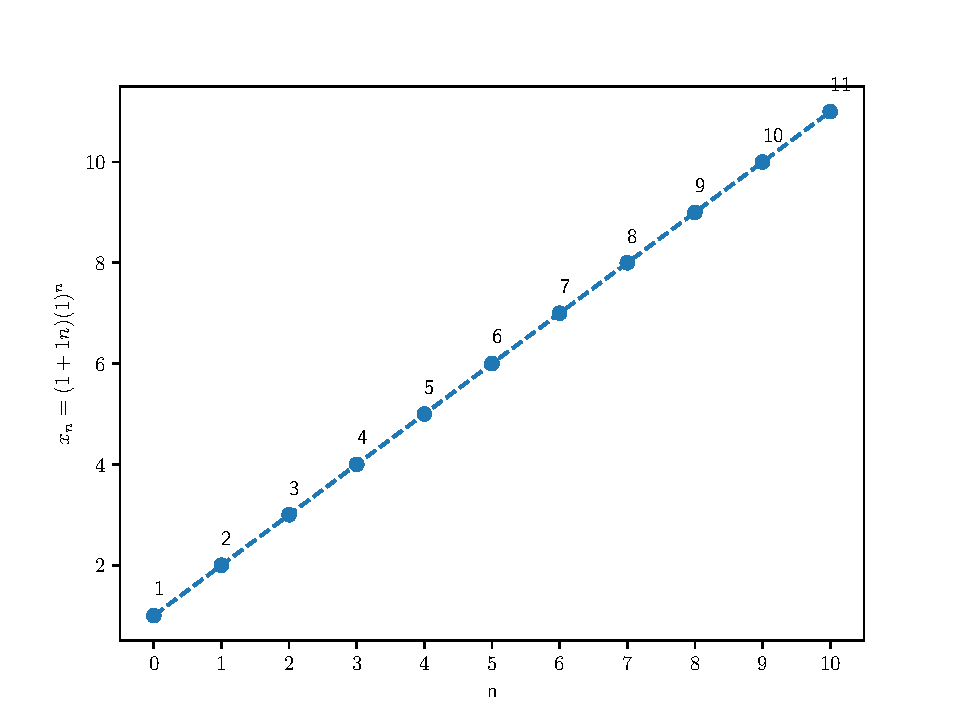
\includegraphics[scale=0.5]{media/hw1/fig3(b)(ii).pdf}
        \end{Figure}

    % Solution 3(b)(iii)
        \item The system of linear difference equation can be written in matrix form: \[
            \left(\begin{matrix}A_1\lambda^{n+1}\\ A_2\lambda^{n+1}\end{matrix}\right)
            = \left(\begin{matrix}
                -3 & -2 \\
                 2 &  1
            \end{matrix}\right)
            \left(\begin{matrix}A_1\lambda^n \\ A_2 \lambda^n \end{matrix}\right)
        \qquad \Leftrightarrow \qquad
            \left(\begin{matrix}
                -3-\lambda & -2 \\
                 2 &  1-\lambda
            \end{matrix}\right) \left(\begin{matrix}A\\B\end{matrix}\right)
            = 0
        \]
        Let determinant of the matrix of coefficients euqal to $0$, it leads to \[
            \mathbf{det}\left(\begin{matrix}
                -3-\lambda & -2 \\
                 2 &  1-\lambda
            \end{matrix}\right) = 0 \qquad \Rightarrow \qquad
            \lambda^2 + 2\lambda + 1 = 0
        \]
        So we hanve two repeated eigenvalues $\lambda_1 = \lambda_2 = \lambda = -1$. And the
        general solution would be \[
            x_n = (A_1 + A_2 n) (-1)^n,
        \]
        \begin{Figure}
            \centering
            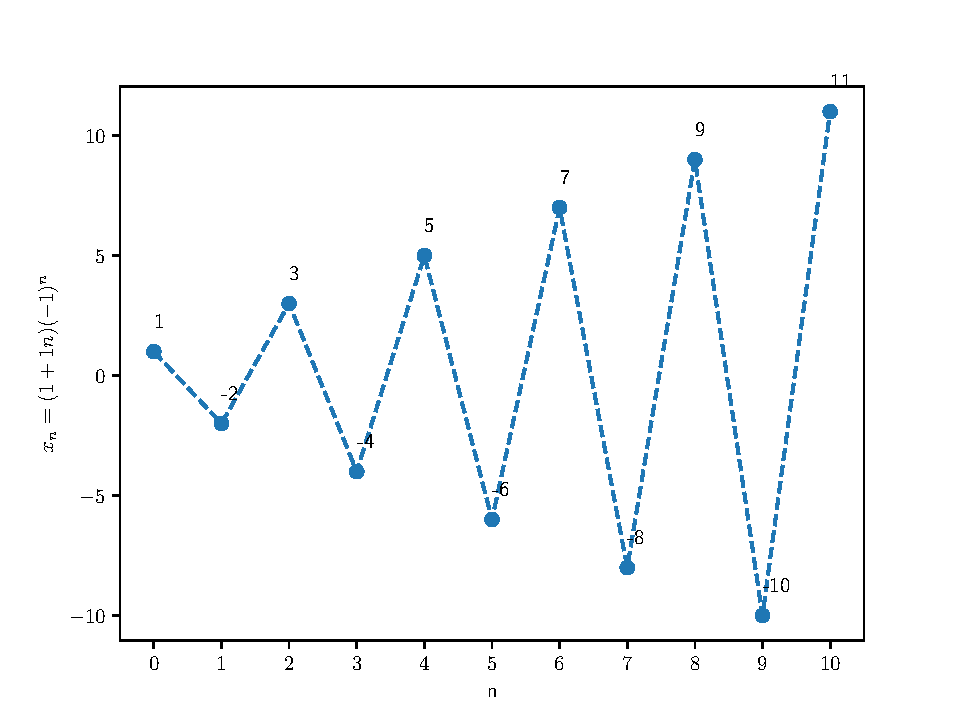
\includegraphics[scale=0.5]{media/hw1/fig3(b)(iii).pdf}
        \end{Figure}
    \end{enumerate}
\end{enumerate}
\end{homeworkProblem}

\pagebreak

% Problem 4
\begin{homeworkProblem}
In Section 1.4 we determined that there are two values $\lambda_1$ and
$\lambda_2$ and two vectors $\left(\begin{matrix}A_1\\B_1\end{matrix}\right)$
and $\left(\begin{matrix}A_2\\B_2\end{matrix}\right)$ called
\textit{eigenvectors} that satisfy equation (29).

\begin{enumerate}
    \item Show that this equation can be written in matrix form as
    \[
    \lambda\left(\begin{matrix}
        A\\B
    \end{matrix}\right) = \mathbf{M} \left(\begin{matrix}
        A\\B
    \end{matrix}\right)
    \]
    where $\mathbf{M}$ is given by equation (27c).
    \item Show that one way of expressing the eigenvectors in terms of $a_{ij}$
    is: \[
        \left(\begin{matrix}
            A_i\\B_i
        \end{matrix}\right) = \left(\begin{matrix}
            1\\ \frac{\lambda_i - a_{11}}{a_{12}}
        \end{matrix}\right)
    \]
    for $a_{12} \neq 0$.
    \item Show that eigenvectors are defined only up to a multiplicative
    constant; i.e., if $\mathbf{v}$ is an eigenvector corresponding to the
    eigenvalue $\lambda$, then $\alpha\mathbf{v}$ is also an eigenvector
    corresponding to $\lambda$ for all real numbers $\alpha$.
\end{enumerate}

\segline

\solution
\begin{enumerate}
    \item Equation (29) in the book is \[
        \begin{aligned}
            0 &= A(a_{11} - \lambda) + B(a_{12})\\
            0 &= A(a_{21}) + B(a_{22} - \lambda)
        \end{aligned}
    \]
    Re-arranging the terms with $\lambda$ to the left-hand side gives\[
        \begin{aligned}
            \lambda A &= a_{11} A + a_{12} B\\
            \lambda B &= a_{21} A + a_{22} B
        \end{aligned}
    \]
    which is equivalent of \[
        \lambda \left(\begin{matrix}
            A\\B
        \end{matrix}\right) = \left(\begin{matrix}
            a_{11} & a_{12}\\
            a_{21} & a_{22}
        \end{matrix}\right) \left(\begin{matrix}
            A\\B
        \end{matrix}\right) = \mathbf{M} \left(\begin{matrix}
            A\\B
        \end{matrix}\right)
    \]
    \item \textit{Proof}. Suppose the eigenvalue is $\lambda_i$ and the
    eigenvector corresponding to it is $\mathbf{v}_i = \left(\begin{matrix}
        A_i\\B_i
    \end{matrix}\right)$. Then we know by the definition of eigenvector that \[
        \left(\begin{matrix}
            a_{11} & a_{12}\\
            a_{21} & a_{22}
        \end{matrix}\right) \mathbf{v}_i = \lambda_i \mathbf{v}_i.
    \]
    Suppose $\mathbf{v}_i = \left(\begin{matrix}
        1\\
        \frac{\lambda_i - a_{11}}{a_{12}}
    \end{matrix}\right)$, then\[
        \left(\begin{matrix}
            a_{11} & a_{12}\\
            a_{21} & a_{22}
        \end{matrix}\right) \mathbf{v}_i =
        \left(\begin{matrix}
            a_{11} & a_{12}\\
            a_{21} & a_{22}
        \end{matrix}\right)
        \left(\begin{matrix}
            1\\ \frac{\lambda_i - a_{11}}{a_{12}}
        \end{matrix}\right) =
        \left(\begin{matrix}
            \lambda_i \\
            a_{21} + \frac{a_{22}(\lambda_i - a_{11})}{a_{12}}
        \end{matrix}\right)
    \]
    And \[
        \lambda_i \mathbf{v}_i = \left(\begin{matrix}
            \lambda_i \\
            \frac{\lambda_i^2 - a_{11}\lambda_i}{a_{12}}
        \end{matrix}\right)
    \]
    Suppose \[
        \left(\begin{matrix}
            \lambda_i \\
            a_{21} + \frac{a_{22}(\lambda_i - a_{11})}{a_{12}}
        \end{matrix}\right) = \left(\begin{matrix}
            \lambda_i \\
            \frac{\lambda_i^2 - a_{11}\lambda_i}{a_{12}}
        \end{matrix}\right)
    \]
    since we have $a_{12} \neq 0$, there will be \[
        \lambda_i^2 -a_{11}\lambda_i =
        a_{21}a_{12} + a{22} \lambda_i - a+{11}a_{22}
    \]
    which gives \[
        \lambda_i = \frac{\beta \pm \sqrt{\beta^2 - 4\gamma}}{2}
    \]
    where \[
        \beta = a_{11} + a_{22}, \quad \gamma = (a_{11}a_{22} - a_{21}a_{12}).
    \]
    And that's exactly the value of $\lambda_i$.

    Thus we have shown that $\mathbf{v}_i = \left(\begin{matrix}
        1\\ \frac{\lambda_i - a_{11}}{a_{12}}
    \end{matrix}\right)$ satisfies
    $\mathbf{M}\mathbf{v}_i = \lambda_i \mathbf{v}_i$,
    i.e. it is indeed one way of expressing the eigenvector.
    \begin{flushright}
        $\qed$
    \end{flushright}

    \item \textit{Proof}. Suppose that $\mathbf{v}$ is the eigenvector
    corresponding to eigenvalue
    $\lambda$, then it is known that \[
        \mathbf{M}\mathbf{v} = \lambda\mathbf{v}
    \]
    For $\alpha\mathbf{v}$, we know from the properties of scalar multiplication
    \[
        \mathbf{M} \left(\alpha \mathbf{v}\right) =
        \alpha \left(\mathbf{M} \mathbf{v}\right)
    \]
    and \[
        \lambda(\alpha\mathbf{v}) = \alpha(\lambda \mathbf{v})
    \]
    It's clear that the two quantities are equal. Thus, by the definition of
    eigenvectors, $\alpha \mathbf{v}$ is also an eigenvector.
    \begin{flushright}
        $\qed$
    \end{flushright}
\end{enumerate}
\end{homeworkProblem}

\pagebreak

\addtocounter{homeworkProblemCounter}{3}

% Problem 8
\begin{homeworkProblem}
The following complex numbers are expressed as $\lambda=a+bi$, where $a$ is the
real part and $b$ is the imaginary part. Express the nubmer in polar form
$\lambda = re^{i\theta}$, and use your result to compute the indicated power
$\lambda^n$ of this complex number. Sketch $\lambda^n$, for $n = 0, 1, 2, 3, 4$
as a function of $n$.
\begin{multicols}{2}
    \begin{enumerate}
        \item $1+i$
        \item $1-i$
        \item $10i$
        \item $-1+\sqrt{3}i$
        \item $-\frac{1}{2} - \frac{i}{2}$
        \item[\vspace{\fill}] % placeholder
    \end{enumerate}
\end{multicols}

\segline

\solution

\begin{multicols}{2}
\begin{enumerate}

% Solution 8(a)
\item \textbf{Polar form}:
$\begin{aligned}
    z^n &= (\sqrt{1^2 + 1^2} e^{i\tan^{-1}(1)})^n\\ &= (\sqrt{2})^n e^{i\pi n/4}
\end{aligned}$.
\begin{Figure}
    \centering
    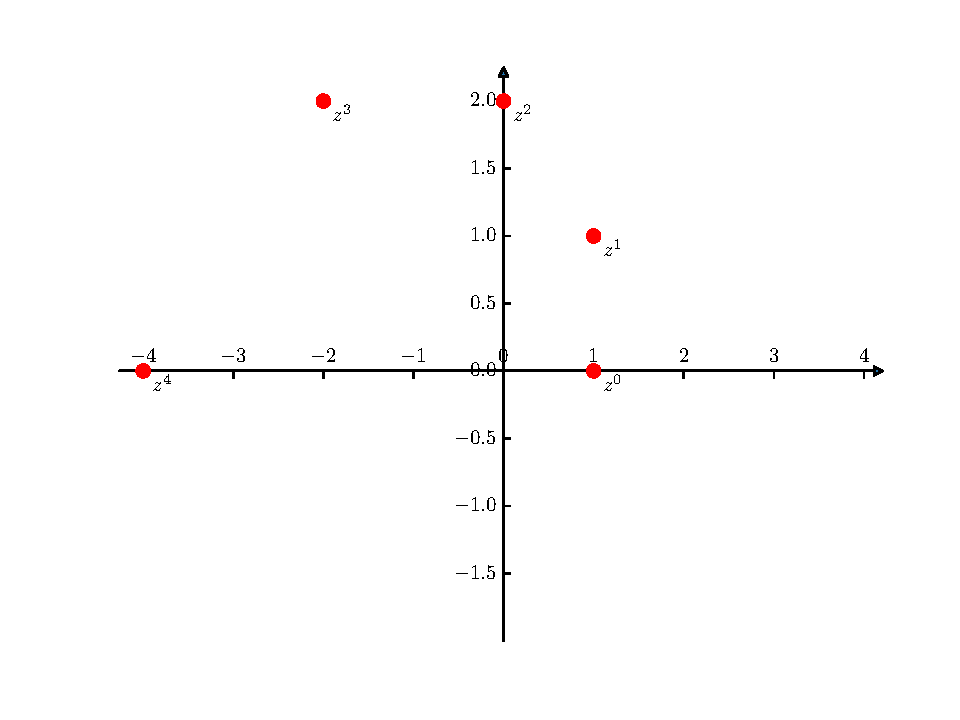
\includegraphics[scale=0.5]{media/hw1/fig8(a).pdf}
\end{Figure}

% Solution 8(b)
\item \textbf{Polar form}:
$\begin{aligned}
    z^n &= (\sqrt{1^2 + (-1)^2} e^{i\tan^{-1}(-1)})^n\\
    &= (\sqrt{2})^n e^{-i\pi n/4} (\cos > 0\& \sin < 0)
\end{aligned}$.
\begin{Figure}
    \centering
    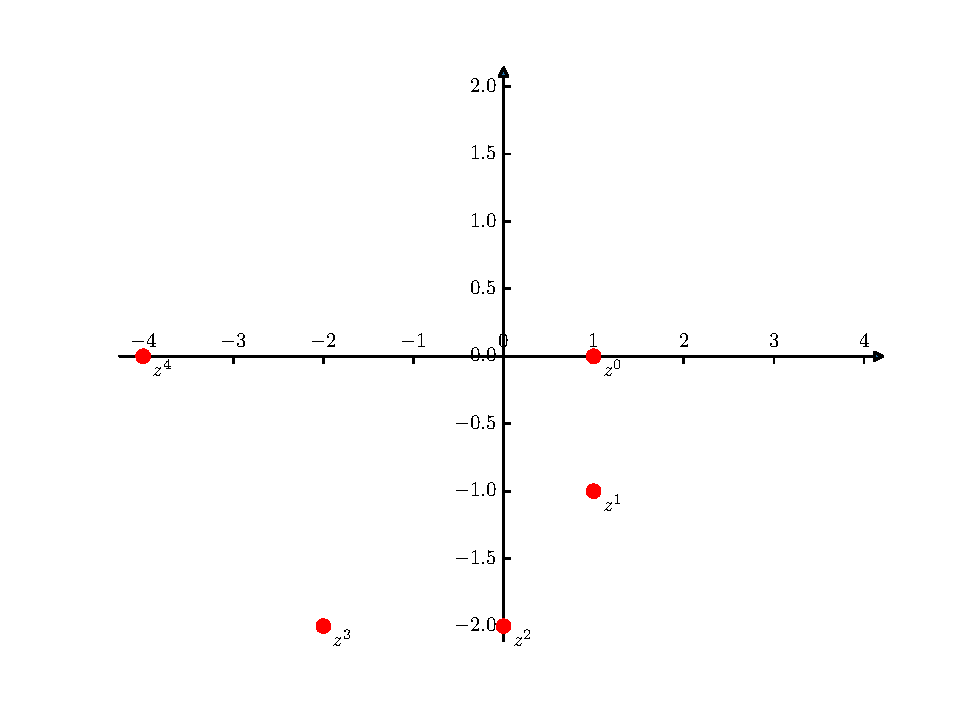
\includegraphics[scale=0.5]{media/hw1/fig8(b).pdf}
\end{Figure}

% Solution 8(c)
\item \textbf{Polar form}:
$\begin{aligned}
    z^n &= (\sqrt{0^2 + 10^2} e^{i\tan^{-1}(10/0)})^n\\ &= 10^ne^{i\pi n/2}
\end{aligned}$.
\begin{Figure}
    \centering
    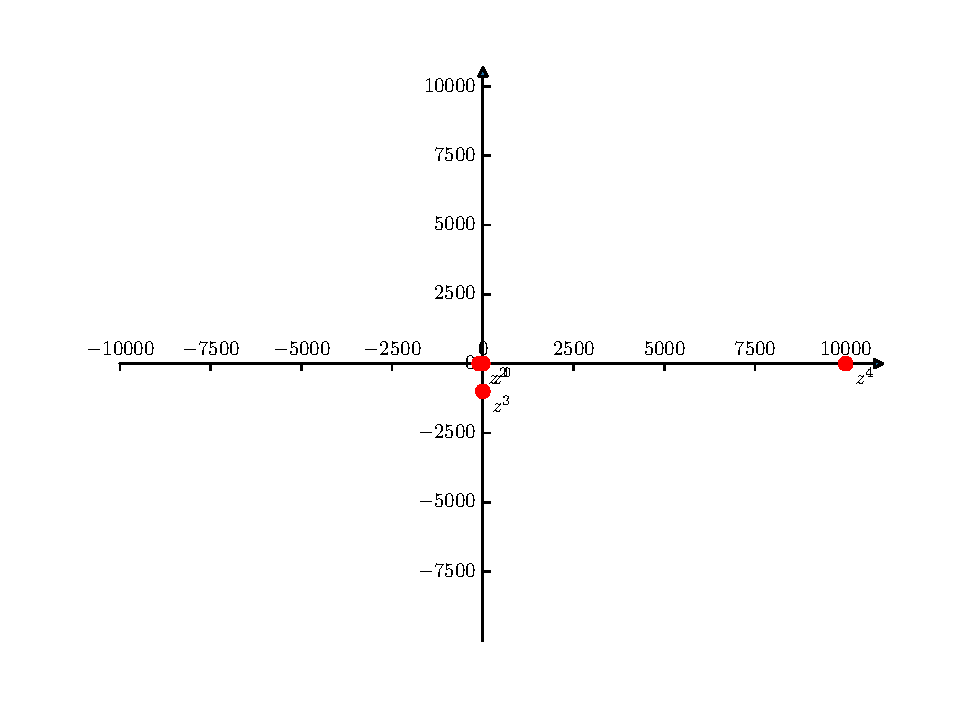
\includegraphics[scale=0.5]{media/hw1/fig8(c).pdf}
\end{Figure}

% Solution 8(d)
\item \textbf{Polar form}:
$\begin{aligned}
    z^n &= (\sqrt{(-1)^2 + (\sqrt{3})^2} e^{i\tan^{-1}(-\sqrt{3})})^n\\
    &= 2^n e^{2i\pi n/3}
\end{aligned}$
\begin{Figure}
    \centering
    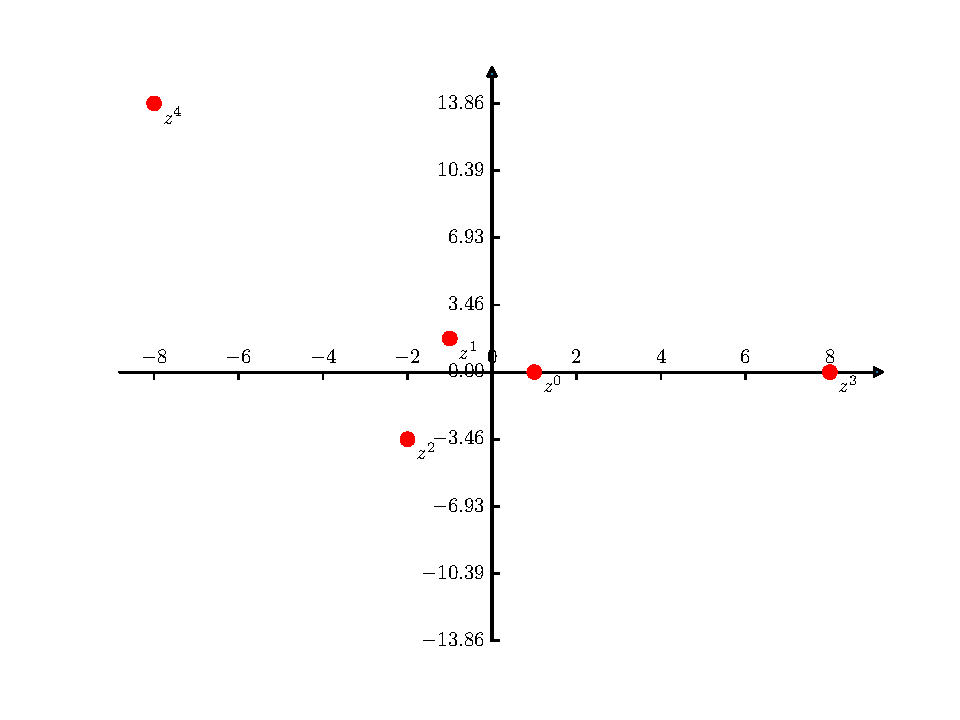
\includegraphics[scale=0.5]{media/hw1/fig8(d).pdf}
\end{Figure}
% Solution 8(e)
\item \textbf{Polar form}:
$\begin{aligned}
    z^n &= (\sqrt{(-1/2)^2+(-1/2)^2} e^{i\tan^{-1}(1)})^n\\
    &=(\frac{1}{\sqrt{2}})^n e^{i5\pi n/4} (\sin \& \cos < 0)
\end{aligned}$.
\begin{Figure}
    \centering
    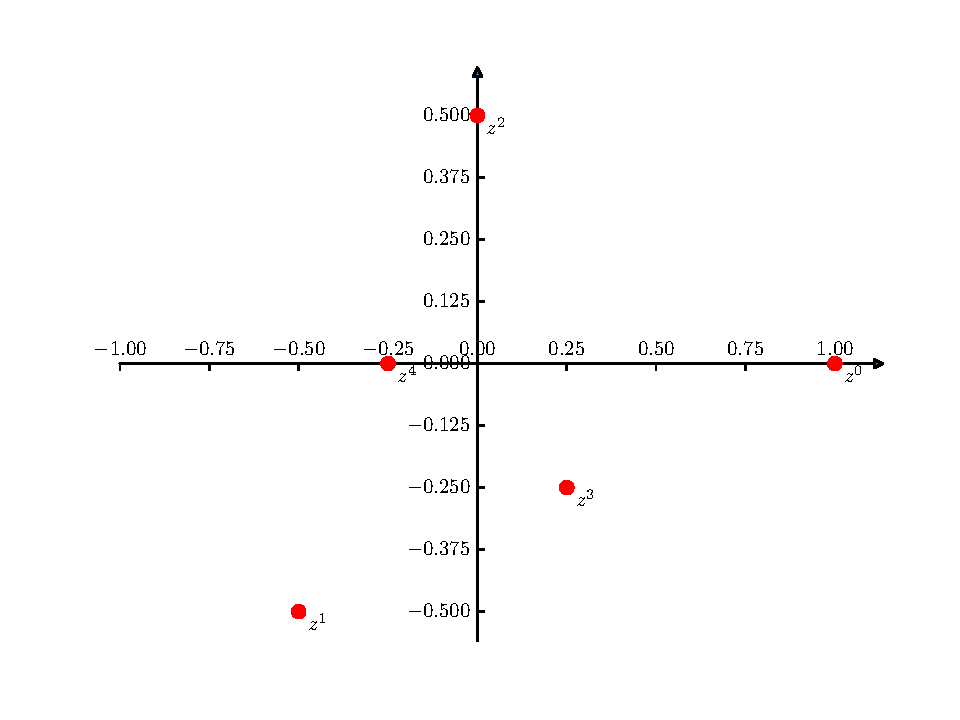
\includegraphics[scale=0.5]{media/hw1/fig8(e).pdf}
\end{Figure}

\end{enumerate}
\end{multicols}
\end{homeworkProblem}

% Problem 9
\begin{homeworkProblem}
\textit{Complex eigenvalues}. Solve and graph the  solutions to the following
difference equations.
\begin{enumerate}
    \item $x_{n+2} + x_n = 0$,
    \item $x_{n+2} - x_{n+1} + x_n = 0$,
\end{enumerate}

\segline

\solution

\begin{enumerate}
    % Solution 9(a)
    \item The characterictic equation is \[
        \lambda^2 + \lambda = 0,
    \]
    with the complex conjugate roots $\lambda = 0 \pm i$. Thus $a=0$ and $b=1$,
    so that \[
        \begin{aligned}
            r = \sqrt{a^2 + b^2} = 1,\\
            \theta = \tan^{-1}(1/0) = \pi/2.
        \end{aligned}
    \]
    Thus the real-valued solution is \[
        x_n = C_1 \cos (n\pi/2) + C_2 \sin (n\pi/2)
    \]
    \begin{Figure}
        \centering
        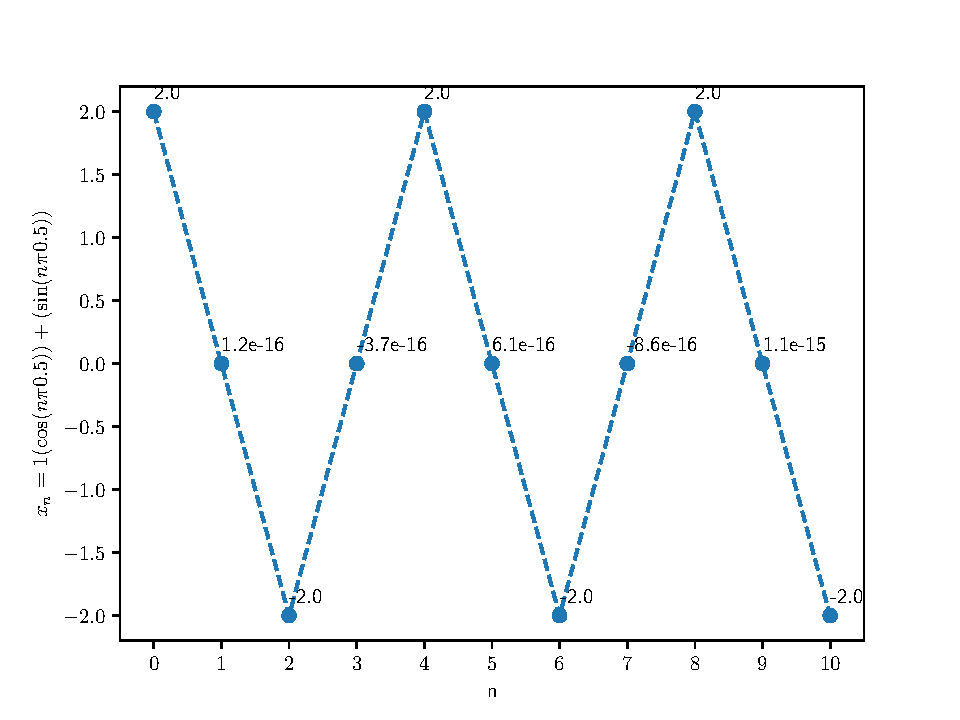
\includegraphics[scale=0.5]{media/hw1/fig9(a).pdf}
    \end{Figure}

    % Solution 9(b)
    \item The characterictic equation is \[
        \lambda^2 - \lambda + 1 = 0,
    \]
    with the complex conjugate roots
    $\lambda = \frac{1}{2} \pm \frac{\sqrt{3}}{2}i$.
    Thus $a = \frac{1}{2}$ and $b = \frac{\sqrt{3}}{2}$,
    so that \[
        \begin{aligned}
            r = \sqrt{a^2 + b^2} = 1,\\
            \theta = \tan^{-1}(b/a) = \pi/3.
        \end{aligned}
    \]
    Thus the real-valued solution is \[
        x_n = C_1 \cos (n\pi/3) + C_2 \sin (n\pi/3)
    \]
    \begin{Figure}
        \centering
        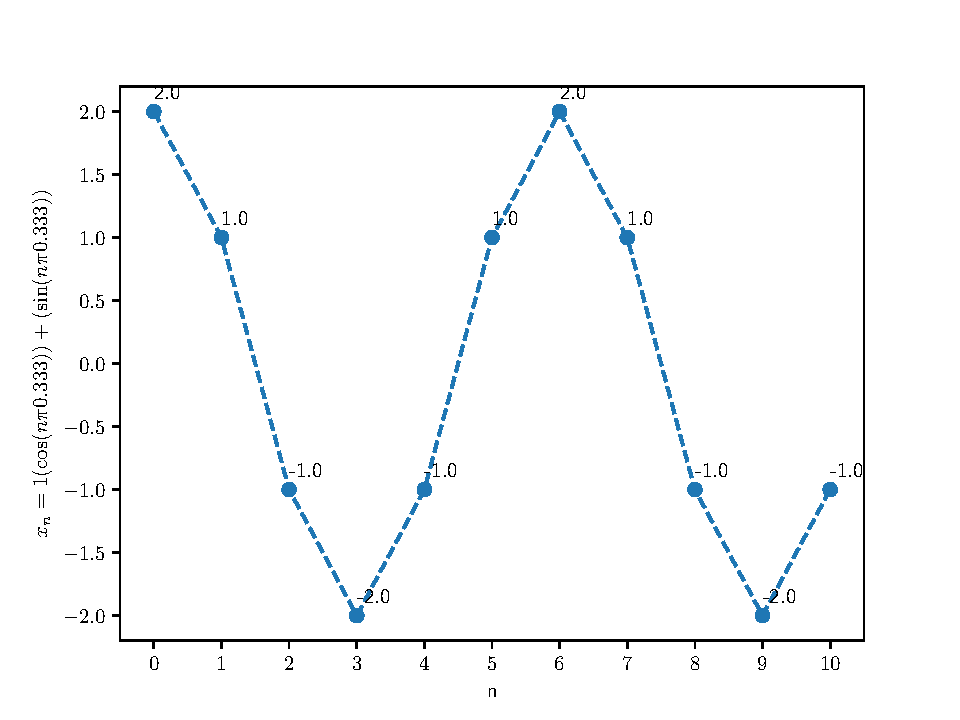
\includegraphics[scale=0.5]{media/hw1/fig9(b).pdf}
    \end{Figure}

\end{enumerate}
\end{homeworkProblem}

% Problem 10
\begin{homeworkProblem}
\begin{enumerate}
    \item Consider the growth of an aphid population described in Section 1.1.
    If the fractional mortality of aphids is 80\% and the sex ratio (ratio of
    females to the total number of aphids) is 50\%, what minimum fecundity $f$
    is required to prevent extinction.
    \item Establish a general condition on the fecundity of aphids to guarantee
    population growth given a fixed survivorship and a known sex ratio.
\end{enumerate}

\segline

\solution

\begin{enumerate}
    \item Extinction will be prevented if the growth rate $\lambda = rf(1-m)>1$.
    Solving the inequity by plugging in given values gives $f = 10$, i.e. a
    fecundity of 10 progeny per female.
    \item In general, we need $f \geq \frac{1}{r(1-m)}$
\end{enumerate}

\end{homeworkProblem}

\pagebreak

% ---------------------------------------------------------------------------- %

\begin{center}
    \LARGE
    \textbf{BIO PART}
\end{center}

\addtocounter{homeworkProblemCounter}{5}

% Problem 16
\begin{homeworkProblem}[][Red blood cell production]
\begin{enumerate}
% Solution 16(a)
\item We have \begin{align}
    R_{n+1} &= (1-f) R_n + M_n, \label{eq:RBC_in_circulation}\\
    M_{n+1} &= \gamma f R_n \label{eq:RBC_produced_nextgen}
\end{align}
Equation \eqref{eq:RBC_produced_nextgen} can be re-written into \begin{equation}
    M_{n} = \gamma f R_{n-1} \label{eq:RBC_produced}
\end{equation}
Substitute \eqref{eq:RBC_produced} into \eqref{eq:RBC_in_circulation}, we'll get
\[
    R_{n+1} = (1-f) R_n + \gamma f R_{n-1}
\]

% Solution 16(b)
\item From (a), it's easy to see that the characteristic function is \[
    \lambda^2 - (1-f) \lambda - \gamma f
\]
Hence, the eigenvalues are indeed given by \[
    \lambda_{1,2} = \frac{(1-f) \pm \sqrt{(1-f)^2} + 4\gamma f}{2}
\]
Since $f$ is definitely a fraction value between $0$ and $1$ (it's horrible to
think that your spleen removes 100\% of your RBCs in circulation), and $\gamma$
is larger than $0$, so that there will be RBC produced.

Observe the boundary stated above, which makes the model biologically reasonable
, we know \[
    \sqrt{(1-f)^2 + 4\gamma f} > \sqrt{(1-f)^2} = (1-f)
\]
Therefore, we should have a positive and a negative eigenvalue, i.e.,
$\lambda_1 > 0$ and $\lambda_2 < 0$.

% Solution 16(c)
\item Suppose the positive eigenvalue $\lambda_1 = 1$, then \[
    \begin{aligned}
    \frac{(1-f) + \sqrt{(1-f)^2} + 4\gamma f}{2} &= 1\\
    \sqrt{(1-f)^2} + 4\gamma f &= 1+f\\
    (1-f)^2 + 4\gamma f &= (1+f)^2\\
    4\gamma f &= 4f\\
    \gamma &= 1
    \end{aligned}
\]

% Solution 16(d)
\item From (c) we know $\gamma = 1$, so \[
    \sqrt{(1-f)^2} + 4\gamma f = 1+f
\]
Then \[
    \lambda_2 = -2f/2 = -f
    \]
And the solution \[
    R_n = A \lambda_1^n + B \lambda_2^n = A + B(-f)^n
\]
The solution will oscillate around constant $A$, and since $f$ is a fraction the
oscillation amplitude will decrease as $n$ increases. This means that the RBC
number in circulation will eventually reach an equilibrium.
\end{enumerate}
\end{homeworkProblem}

% Problem 17
\begin{homeworkProblem}[][Annual plant propagation]
\begin{enumerate}
    % Solution 17(a)
    \item The model for annual plants was condensed into a single equation (15)
    for $p_n$, the number of plants. Show that it can also be written as a
    single equation in $S_n^1$.

    \textit{Solution}: We have \begin{align}
        &p_n = \alpha s_n^1 + \beta s_n^2 \label{eq:pn} \\
        &\overline{s_n^1} = (1-\alpha)s_n^1 \label{eq:no_germ}\\
        &\overline{s_n^2} = (1-\alpha)s_n^2\\
        &s_n^0=\gamma p_n \label{eq:new_seeds}\\
        &s_{n+1}^1 = \sigma s_n^0 \label{eq:next_gen_seeds_1}\\
        &s_{n+1}^2 = \sigma \overline{s_n^1} \label{eq:next_gen_seeds_2}
    \end{align}

    Make several substitutions:
    \begin{align}
        &\eqref{eq:new_seeds} \rightarrow \eqref{eq:next_gen_seeds_1}
        & & S_{n+1}^1 = \sigma \gamma p_n \label{eq:sn1_next} \\
        % -------------------------------------------------------------------- %
        &\eqref{eq:no_germ} \rightarrow \eqref{eq:next_gen_seeds_2}
        & & S_{n}^2 = \sigma (1-\alpha) S_{n-1}^1 \label{eq:sn2}\\
        % -------------------------------------------------------------------- %
        &\eqref{eq:pn} \rightarrow \eqref{eq:sn1_next}
        & & S_{n+1}^1 = \sigma \gamma (\alpha s_n^1 + \beta s_n^2)
        \label{eq:res}\\
        % -------------------------------------------------------------------- %
        &\eqref{eq:sn2} \rightarrow \eqref{eq:res}
        & & S_{n+1}^1 = \sigma \gamma (\alpha s_n^1 +
        \beta \sigma (1-\alpha) S_{n-1}^1) \label{eq:sol}
    \end{align}
    And equation \eqref{eq:sol} should be the answer.
    % Solution 17(b)
    \item Seeds produced this year (year $n$) which survived the winter and will
    germinate next year (year $(n+1)$)

    % Solution 17(c)
    \item We know from the book that \[
        \lambda_{1,2} = \frac{\sigma \gamma \alpha}{2} (1 \pm \sqrt{1 + \delta})
    \] where \[
        \delta = \frac{4}{\gamma}\frac{\beta}{\alpha}
                \left( \frac{1}{\alpha} - 1\right)
    \]
    We know that $\delta$ is a positive quantity since $\alpha < 1$. So we have
    a positive eigenvalue and a negative eigenvalue.

    If we want the population to increase in size, we should have the positive
    eigenvalue $\lambda_1 > 1$.

    Plug in $\alpha = \beta = 0.001$ and $\sigma = 1$, we'll have \[
    \begin{aligned}
        \delta &= \frac{4}{\gamma}(\frac{1}{0.001} - 1) \approx \frac{4000}{\gamma}\\
        \lambda_1 &= \frac{0.001\gamma}{2} (1 + \sqrt{1 + \delta})
    \end{aligned}
    \quad\rightarrow\quad
    \lambda_1 = \frac{\gamma}{2000}(1 + \sqrt{1+ \frac{4000}{\gamma}}) > 1
    \]
    Solving the inequity gives \[
        \gamma > 500
    \]

    % Solution 17(d)
    \item In case (1), the parameters are: \[
        \alpha = 0.5, \quad \beta = 0.25, \quad \gamma = 2.0, \quad \sigma = 0.8,
    \] we can compute that \[
    \begin{aligned}
        \delta &= \frac{4}{\gamma}\frac{\beta}{\alpha}
        \left( \frac{1}{\alpha} - 1\right)
        = 1\\
        \lambda_1 &= \frac{\sigma \gamma \alpha}{2} (1 + \sqrt{1 + \delta})
        = 0.4 (1 + \sqrt{2})\\
        &\approx 0.97 < 1
    \end{aligned}
    \]
    So the population decreases.

    An in case (2), the parameters are: \[
        \alpha = 0.6, \quad \beta = 0.3, \quad \gamma = 2.0, \quad \sigma = 0.8,
    \] we can compute that \[
    \begin{aligned}
        \delta &= \frac{4}{\gamma}\frac{\beta}{\alpha}
        \left( \frac{1}{\alpha} - 1\right)
        = \frac{2}{3}\\
        \lambda_1 &= \frac{\sigma \gamma \alpha}{2} (1 + \sqrt{1 + \delta})
        = 0.48 (1 + \sqrt{5/3})\\
        &\approx 1.10 >1
    \end{aligned}
    \]
    So the population increases.

    % Solution 17(3)
    \item Consider the positive eigenvalue as \[
        \lambda_1 = \frac{a + \sqrt{a^2 + 4b}}{2}
    \] where \[
        a = \alpha \sigma \gamma, \quad b = \beta \sigma^2 (1-\alpha)\gamma
    \]
    If we want $\lambda_1 > 1$, then \[
    \begin{aligned}
        \frac{a + \sqrt{a^2 + 4b}}{2} &> 1\\
        \sqrt{a^2 + 4b} &> 2-a\\
        a^2 + 4b  &> a^2 - 4a + 4\\
        a + b &> 1
    \end{aligned}
    \] (Note: If $(2-a) < 0$ then the inequity will always be trivially true,
    thus it's not of too much interest. We only consider $(2-a) > 0$ here.)
    Substitute back $a = \alpha \sigma \gamma$ and
    $b = \beta \sigma^2 (1-\alpha)\gamma$, we'll have \[
        \gamma > \frac{1}{\alpha \sigma + \beta \sigma^2 (1-\alpha)}
    \]
\end{enumerate}
\end{homeworkProblem}

\pagebreak

% Problem 18
\begin{homeworkProblem}[][Blood $CO_2$ and ventilation]
\begin{enumerate}
% Solution 18(a)
\item We know from the book that \begin{align}
    C_{n+1} &= C_{n} - \mathcal{L}(V_n, C_n) + m, \label{CO2_next}\\
    V_{n+1} &= \mathcal{S}(C_n). \label{ventilation_next}
\end{align}
From the question description we know that \[
    \mathcal{L}(V_n, C_n) = \beta V_n, \qquad V_{n+1} = \alpha C_n
\]
Make some simple substitution, we'll have \[
    C_{n+1} = C_{n} - \alpha \beta C_{n-1} + m
\]
i.e. \[
    C_{n+1} - C_n + \alpha\beta C_{n-1} = m
\]

% Solution 18(b)
\item \begin{enumerate}[label=(\arabic*)]
% Solution 18(b)(1)
\item Suppose $C_n = m / \alpha \beta$, then \[
    C_{n+1} - C_n + \alpha \beta C_{n-1}
    = m/\alpha\beta - m/\alpha\beta + \alpha\beta \cdot \frac{m}{\alpha\beta}
    = m
\]
Hence, $C_n = m/\alpha \beta$ is a particular solution.
% Solution 18(b)(2)
\item Let $m = 0$, then it'll turn into a homogeneos problem. The characteristic
equation would be \[
    \lambda^2 - \lambda + \alpha\beta = 0
\]
with eigenvalues \[
    \lambda_{1,2} = \frac{1 \pm \sqrt{1 - 4\alpha\beta}}{2},
\]
which is the \textit{complementary/homogeneous solution}.

Combined the complementary solution with the particular solution, the general
solution would be \[
    C_{n} = \frac{m}{\alpha\beta} +
            C_1 \left(\frac{1 + \sqrt{1 - 4\alpha\beta}}{2}\right)^n +
            C_2 \left(\frac{1 - \sqrt{1 - 4\alpha\beta}}{2}\right)^n
\]
\end{enumerate}% end 18(b)

% Solution 18(c)
\item \begin{enumerate}[label=(\arabic*)]
% Solution 18(c)(1)
\item Assume that $4\alpha\beta < 1$, then $\alpha\beta < 1/4$. This implies \[
    \mathcal{L}(V_n, C_n) = \beta V_n = \alpha \beta C_{n-1} < \frac{C_{n-1}}{4}
\]
i.e., the amount of $CO_2$ loss / breathed out will not be larger than
$\frac{1}{4}$ of the blood $CO_2$ amount.

And, since $4 \alpha\beta < 1$, then $ 0 < \sqrt{1 - 4\alpha\beta} < 1$. Let
$\sqrt{1 - 4\alpha\beta} = \delta$, then \[
\begin{aligned}
    \lambda_1 &= \frac{1+\delta}{2} \in (\frac{1}{2}, 1)\\
    \lambda_2 &= \frac{1-\delta}{2} \in (0, \frac{1}{2})
\end{aligned}
\]
Therefore, the absolute value of each eigenvalue $|\lambda_i| < 1$, implying \[
    \lim_{n \to \infty} (C_{n}) = \frac{m}{\alpha\beta}
\] since the power of a fraction will diminish towards $0$.
Under this scenario, a steady state will eventually be established regardless of
 the initial conditions. And the steady ventilation rate would be \[
    V_{n} = \alpha \frac{m}{\alpha\beta} = \frac{m}{\beta}
\]

%Solution 18(c)(2)
\item Assume that $4\alpha\beta > 1$, then $1 - 4\alpha\beta < 0$, which means
that the characteristic equation would have complex eigenvalues. The conjugated
complex eigenvalues $\lambda = a \pm bi$ have \[
    a = \frac{1}{2}, \quad b = \frac{\sqrt{4\alpha\beta - 1}}{2}
\]
i.e. \[
    r = \sqrt{a^2 + b^2} = \sqrt{\alpha\beta}, \quad \theta = \tan^{-1}(b/a)
    = \tan^{-1}(\sqrt{4\alpha\beta - 1})
\]
Then \[
    C_n = r^n (C_1 \cos(n\theta) + C_2 \sin(n\theta))
    = (\sqrt{\alpha\beta})^n \sin(n\theta + \phi)
\]
where $\tan \phi = C_1/C_2$. It is clear that the solution will oscillate at
frequency $f = \theta/2\pi$

If $\alpha\beta \geq 1$, then the oscillation will increase in magnitude. When
$\alpha\beta = 1$, the oscillation frequency would be $f = \tan^{-1}(\sqrt{3}) =
\frac{\pi}{3}$.

This result could correspond to Cheyne-Stokes respiration, which is a disorder
characterized by recurrent oscillation between apnea and hyperpnea (May, 1978
and Naughton, 1998).
\end{enumerate}% end 18(c)

% Solution 18(d)
\item For now the ventilation rate is proportional to blood $CO_2$
concentration. In real biological systems, body will likely adjust the rate of
breath according to $C_n$, just like the relationship between air friction and
velocity. It's suitable to suppose that \[
    \mathcal{S}(C_n) = \alpha C_n^2
\]
Then the equation will turn into \[
    \begin{aligned}
    &C_{n+1} = C_n - \alpha \beta C_{n-1}^2 + m
    &C_{n+1} - C_n + \alpha \beta C_{n-1}^2 = m
    \end{aligned}
\]
Suppose $C_{n+1}=C_n$, then we can derive a steady-state where \[
    C_n = \sqrt{\frac{m}{\alpha\beta}}
\]
It would also be interesting to think about the equilibrium shifting between
bicarbonates and $CO_2$ and the formation of carbaminohemoglobin($HbCO_2$).
But deriving a nice math equation with respect to these factors is out of our
ability.

\end{enumerate}
\end{homeworkProblem}

\pagebreak

\begin{homeworkProblem}[20]
Take $p_n^1$ as the number of newborns, then it should be compute by \[
\begin{aligned}
    p_{n+1}^1 &= \sum^m_{i=1} \left(
        \begin{matrix}
            \text{number of births}\\
            \text{in age class }i\\
            \text{in last year }(n)
        \end{matrix}\right) \left(
        \begin{matrix}
            \text{number of individuals}\\
            \text{in age class }i\\
            \text{in last year }(n)
        \end{matrix}\right)\\
    &= \sum^m_{i=1} \alpha_i p_n^i
\end{aligned}
\]
And for each age class $1< i < m$, it can be computed by \[
    p_{n+1}^i = \sigma_{i-1} p_{n}^{i-1}
\]
Since $m$ is the oldest age class, $p_n^m$ will not survive to next year.
The system of equations can be written in the form of \[
\begin{aligned}
    p_{n+1}^1 &= \alpha_1 p_n^1 + \alpha_2 p_n^2 + \alpha_3 p_n^3 + \cdots
    + \alpha_{m-1} p_n^{m-1} + \alpha_m p_n^m\\
    p_{n+1}^2 &= \sigma_1 p_n^1\\
    p_{n+1}^3 &= \phantom{\sigma_1 p_n^1 + }\ \sigma_2 p_n^2\\
    \vdots &\phantom{=}\\
    p_{n+1}^{m} &=
    \phantom{\alpha_1 p_n^1 + \alpha_2 p_n^2 + \alpha_3 p_n^3 +\cdots\cdots}
    \sigma_{m-1} p_n^{m-1}
\end{aligned}
\]
It's clear that it can be written as the matrix form:
\[
    \mathbf{P}_{n+1} = \mathbf{A} \mathbf{P}_n
\]
where \[
    \mathbf{P}_k = \left(\begin{matrix}
        p_k^1 \\ p_k^2 \\ \vdots \\ p_k^m
    \end{matrix}\right), \qquad
    \mathbf{A} = \left(\begin{matrix}
        \alpha_1 & \alpha_2 & \cdots & \alpha_{m-1} & \alpha_m  \\
        \sigma_1 & 0        & \cdots & 0            & 0         \\
        0        & \sigma_2 & \cdots & 0            & 0         \\
        \vdots   & \vdots   & \ddots & \vdots       & \vdots    \\
        0        & 0        & \cdots & \sigma_{m-1} & 0
    \end{matrix}\right)
\]
\end{homeworkProblem}

\pagebreak

% ---------------------------------------------------------------------------- %

\begin{center}
    \LARGE
    \textbf{CODE PART}
\end{center}

% Problem 6
\begin{homeworkProblem}[6]
\begin{enumerate}
\item \begin{multicols}{2}
As seen in this graph of 6a, each initial condition produces a unique
exponential mapping, however, all the mappings follow the same pattern and are
unstable.
$$
x_{n+2} – 7x_{n+1} + 10x_n = 0
$$

\begin{Figure}
    \centering
    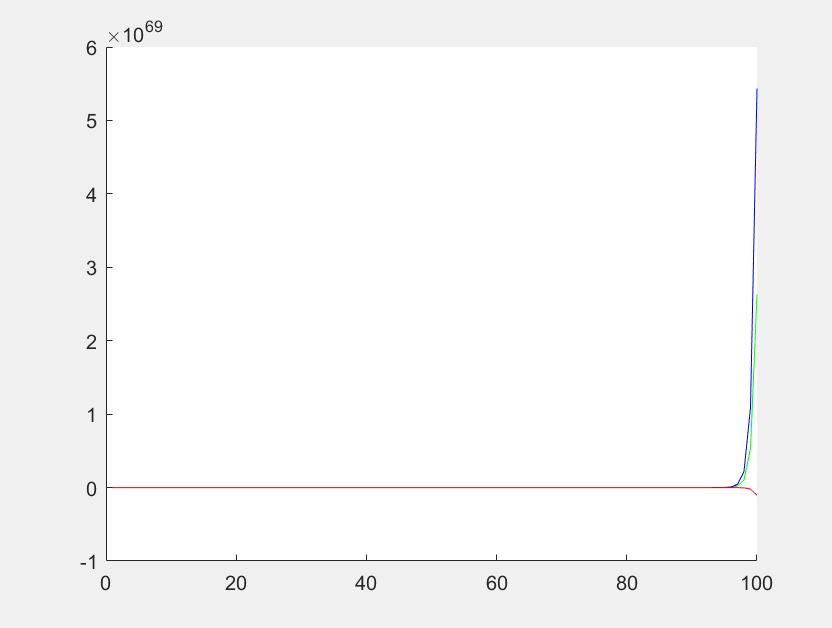
\includegraphics[scale=0.3]{media/hw1/fig6(a).png}
\end{Figure}

\end{multicols}

\begin{listing}[htbp]
    \begin{tcolorbox}
    \begin{minted}{matlab}
clear all
eig1=5;
eig2=2;
x(1)=0;
x(2)=1;
x(3)=0.5;
x(4)=-0.1;
x(5)=2;
x(6)=3;
n=linspace(1,500);
for k=1:2:6
    syms A B
    [solA,solB] = solve(
        A*eig1^x(k) + B*eig2^x(k) == x(k),
        A*eig1^x(k+1) + B*eig2^x(k+1) == x(k+1));
    n=[1:1:100];
    if k == 1
        hold on
        g=solA.*eig1.^n + solB.*eig2.^n;
        plot(n,g,'g')
    elseif k == 3
        hold on
        b=solA.*eig1.^n + solB.*eig2.^n;
        plot(n,b,'b')
    else
        hold on
        r=solA.*eig1.^n + solB.*eig2.^n;
        plot(n,solA.*eig1.^n + solB.*eig2.^n,'r')
    end
end
    \end{minted}
    \end{tcolorbox}
\end{listing}
\pagebreak
\begin{multicols}{2}
(c). As seen in this graph of 6c, each initial condition produces a unique
exponential mapping, however, all the mappings follow the same pattern and are
unstable.
$$
x_{n+2} - \sigma_1 x_{n+1} + \sigma_2 x_n = 0
$$

\begin{Figure}
    \centering
    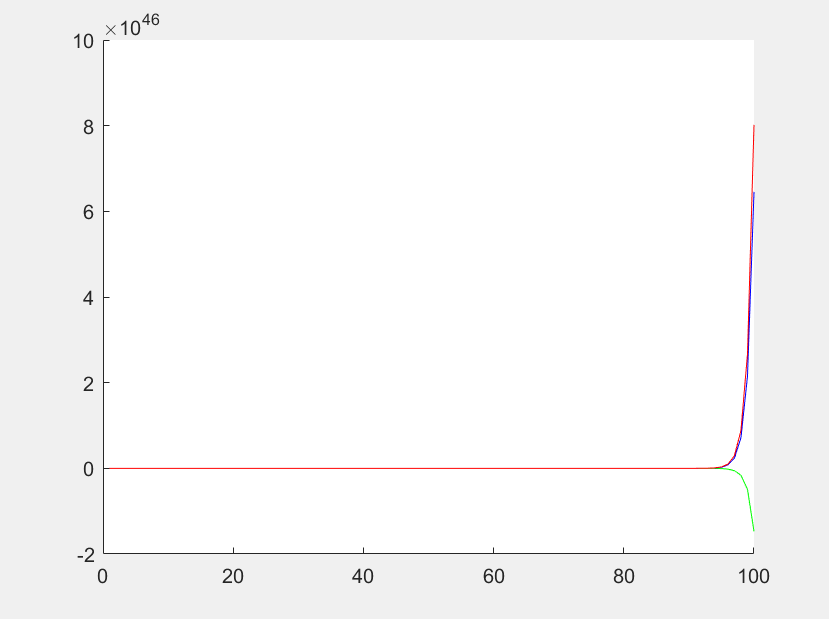
\includegraphics[scale=0.35]{media/hw1/fig6(c).png}
\end{Figure}
\end{multicols}
\begin{listing}[htbp]
    \begin{tcolorbox}
    \begin{minted}{matlab}
clear all
s1= -1;
s2= -2;
beta= 3;
eig1=(1/2)*(-s1+(sqrt(s1^2 -4*s2*beta)))
eig2=(1/2)*(-s1-(sqrt(s1^2 -4*s2*beta)))
x(1)=7;
x(2)=1;
x(3)=0.5;
x(4)=-0.1;
x(5)=2;
x(6)=3;
n=linspace(1,500);

for k=1:2:6
    syms A B
    [solA,solB] = solve(
        A*eig1^x(k) + B*eig2^x(k) == x(k),
        A*eig1^x(k+1) + B*eig2^x(k+1) == x(k+1));
    n=[1:1:100];
    if k == 1
        hold on
        g=solA.*eig1.^n + solB.*eig2.^n;
        plot(n,g,'g')
    elseif k == 3
        hold on
        b=solA.*eig1.^n + solB.*eig2.^n;
        plot(n,b,'b')
    else
        hold on
        r=solA.*eig1.^n + solB.*eig2.^n;
        plot(n,solA.*eig1.^n + solB.*eig2.^n,'r')
    end
end
    \end{minted}
    \end{tcolorbox}
\end{listing}
\pagebreak
\addtocounter{enumi}{4}

\item \begin{multicols}{2}
As seen in this graph of 6f, each initial condition produces a unique
oscillating mapping, however, all the mappings follow the same pattern and are
unstable.
$$
x_{n+2} – \frac{5}{4}x_{n+1} + \frac{11}{8}x_n = 0
$$

\begin{Figure}
    \centering
    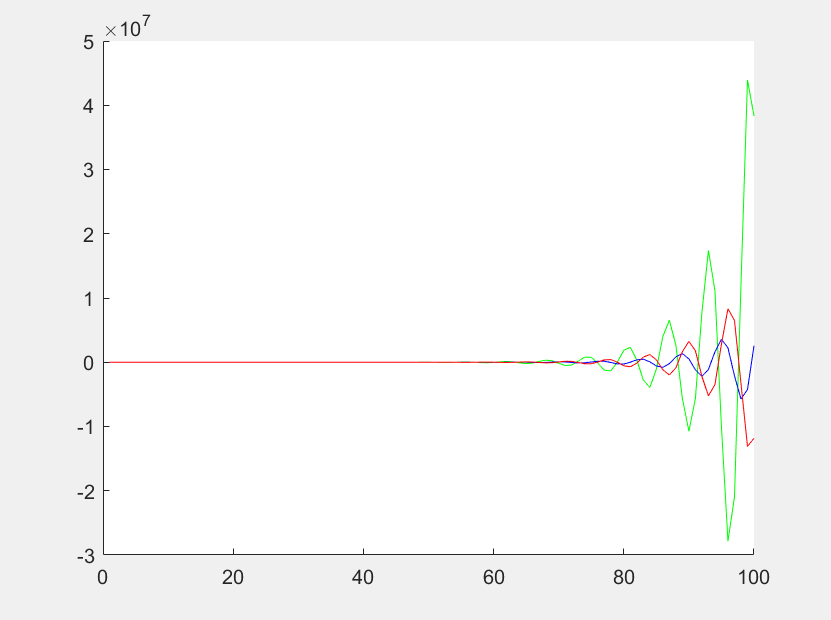
\includegraphics[scale=0.35]{media/hw1/fig6(f).png}
\end{Figure}
\end{multicols}

\begin{listing}[htbp]
    \begin{tcolorbox}
    \begin{minted}{matlab}
clear all
eig1=(1/2)*(1.25+sqrt(1.5625-5.5))
eig2=(1/2)*(1.25-sqrt(1.5625-5.5))
x(1)=7;
x(2)=1;
x(3)=0.5;
x(4)=-0.1;
x(5)=2;
x(6)=3;
n=linspace(1,500);

for k=1:2:6
    syms A B
    [solA,solB] = solve(
        A*eig1^x(k) + B*eig2^x(k) == x(k),
        A*eig1^x(k+1) + B*eig2^x(k+1) == x(k+1));
    n=[1:1:100];
    if k == 1
        hold on
        g=solA.*eig1.^n + solB.*eig2.^n;
        plot(n,g,'g')
    elseif k == 3
        hold on
        b=solA.*eig1.^n + solB.*eig2.^n;
        plot(n,b,'b')
    else
        hold on
        r=solA.*eig1.^n + solB.*eig2.^n;
        plot(n,solA.*eig1.^n + solB.*eig2.^n,'r')
    end
end
    \end{minted}
    \end{tcolorbox}
\end{listing}
\end{enumerate}
\end{homeworkProblem}

\end{document}